\section{Defining Engineering Design}

Over the years, there has been many attempts to define Engineering Design. 
This has been a non-trivial task and is mainly due to the increasingly complex and multi-disciplinary nature of design. 
An element that continue to increase over the years with the rate of technological development.

\marginnote{Fielden Report}In the first two years of the Bath Engineering Degree, we will be focusing on the design of mechanical components, systems and machines. 
Therefore, we will be using Fielden's definition of Engineering Design:

\begin{center}
  ``The use of scientific principles, technical information and imagination in the definition of a mechanical structure, machine or system to perform pre-specified function with the maximum economy and efficiency.''~\cite{fielden1963}
\end{center}

\citeauthor{pahl2013}~\cite{pahl2013} also provides an interesting perspective on Engineering Design and how it forms the bridge between the sciences (\cref{fig-ed}). It is being able to analyse and critique designs both objectively and subjectively, which is key to being a Design Engineer.


\begin{figure*}[h!]
  \centering
  \resizebox{0.8\textwidth}{!}{
      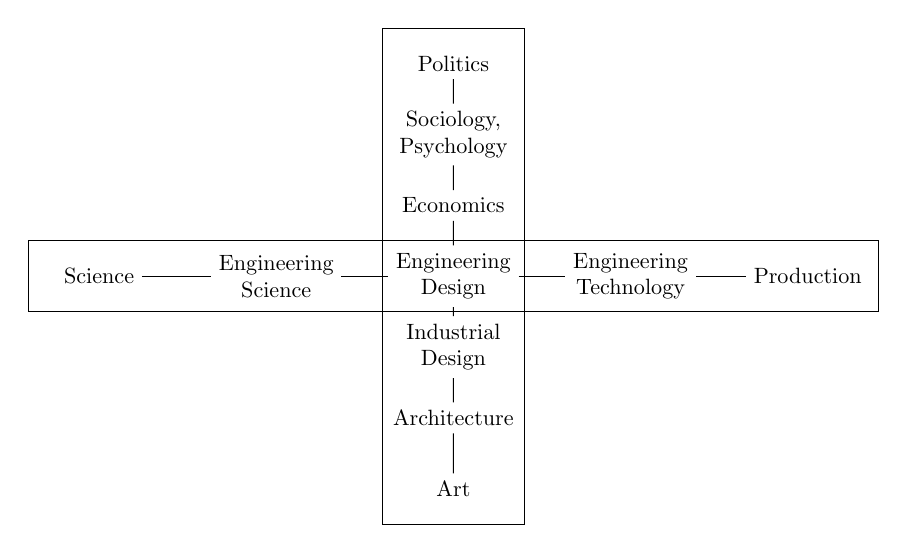
\begin{tikzpicture}[scale=0.9, every node/.style={scale=0.8}]
        \node[align=center] (A) at (0,3) {Politics};
        \node[align=center] (B) at (0,2) {Sociology,\\ Psychology};
        \draw (A) -- (B);
        \node[align=center] (C) at (0,1) {Economics};
        \draw (B) -- (C);
        \node[align=center] (D) at (0,0) {Engineering\\ Design};
        \draw (C) -- (D);
        \node[align=center] (E) at (0,-1) {Industrial\\ Design};
        \draw (D) -- (E);
        \node[align=center] (F) at (0,-2) {Architecture};
        \draw (E) -- (F);
        \node[align=center] (G) at (0,-3) {Art};
        \draw (F) -- (G);
    
        \node[align=center] (H) at (-5,0) {Science};
        \node[align=center] (I) at (-2.5,0) {Engineering\\ Science};
        \draw (H) -- (I);
        \draw (I) -- (D);
    
        \node[align=center] (J) at (5,0) {Production};
        \node[align=center] (K) at (2.5,0) {Engineering\\ Technology};
        \draw (D) -- (K);
        \draw (J) -- (K);
    
        \draw[] (-1,-3.5) rectangle (1,3.5);
        \draw[] (-6,-0.5) rectangle (6,0.5);
    
      \end{tikzpicture}
  }
  \caption[Positioning Engineering Design within the sciences]{Positioning Engineering Design within the sciences~\citep{pahl2013}}\label{fig-ed}
\end{figure*}